\section{Experiment's outputs}
\label{sec:Experimentsoutputs}

Once an experiment is completed, a set of raw images, as well as the corresponding stimuli information and event timings is available. For each protocol, there is a set of frames for every trial, according to the TPLSM system's scanning speed of $30 Hz$ ($6 Hz$ per plane). 
For instance, the RF protocol comprises 1120 trials and the triggers sent from bpod to the imaging computer for separating the movies come at each 4 trials. There are thus, for this case, 280 sets of images. Since each trial endures for $1s$, each of these sets contains 6 frames for each of the 4 relevant planes, prefacing, for the RF protocol, 24 total frames per trial. In turn, each of these frames contains a $512 \times 512$ pixels image of the fluorescent signals emitted from the animal's brain ($200 \mu m \times 200 \mu m$) and detected at that time (figure \ref{cm006}, for an example).
For each of the trial's sets of images, there is the corresponding stimulus information being saved in a Matlab structure: In the case of the RF, the changing feature is the position and the gratings direction order of the stimulus patch being presented in the screen during that trial, for the Tuning protocol these are the spacial and temporal frequencies as well as the direction of the centred stimulus, and finally for the SM protocol the independent variable is the stimulus type number. Apart from these, the constant features of the stimuli at each protocol are also saved in the same stimuli structure. 
The trial time stamps in bpod's triggering, states and Psychtoolbox's clocked timings from a received trigger to the next are also saved. This allows, in the latter analysis, to confirm and correct the stimuli information in the case of any eventual skipped trials.
Finally, Scan Image configurations are also saved, in each trial's video header, keeping the information required about the laser's power during that experiment, multiplane settings and read brightness offsets.

\begin{figure}[H] \centering 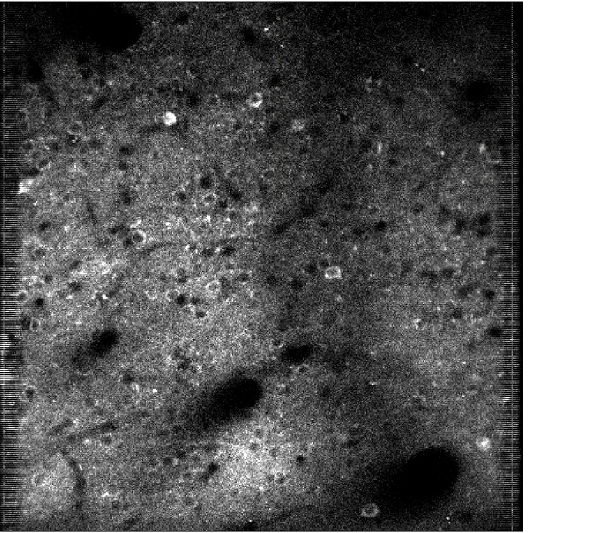
\includegraphics[width=10cm,height=10cm,keepaspectratio]{Figures/7.Results/ftraces/CM006.png} 
\caption{Average image of an example plane of imaging recordings across a session from an example animal. The full image corresponds to a $512\times 512$ map of $200 \mu m \times 200 \mu m$ of mouse V1 area, chosen as to respond to the center of the visual field of view.
\label{cm006}}
\end{figure}